\section{PROLOG} % Necessário para gerar o \tableofcontents

\begin{frame}[t]
\vskip 3cm
\begin{center}
{\Huge Introdução à Programação em Lógica}
\end{center}
\end{frame}

\begin{frame}[t]{Programação em Lógica}
	\begin{itemize}
	\item Programação Lógica é um paradigma de programação baseado em linguagens {\bf declarativas}

	\item Um programa declarativo rompe com a noção de \underline{sequencialidade} de instruções lógicas; ao invés disso, trabalha com os conceitos de conhecimento declarativo e procedimental
	
	\item Conhecimento {\bf declarativo} é aquele conhecimento que é especificado cujo uso não foi definido
	
	\item Conhecimento {\bf procedimental} são informações de controle sobre o uso do conhecimento declarativo	
	\end{itemize}
\end{frame}

\begin{frame}[t]{Programação Lógica}
	\begin{itemize}
	\item O processo de se programar através desse paradigma é o que se segue:
	\end{itemize}
	\begin{enumerate}
	\item Modelagem do(s) domínio(s)
	\item Modelagem dos fatos conhecidos acerca do problema
	\item Modelagem das regras conhecidas acerca do problema
	\item Consulta à base de conhecimento
	\item Especificação da inferência desejada (predicado)
	\end{enumerate}
	
	Em caso de sucesso, o \underline{motor de inferência} retorna o predicado com suas variáveis {\bf unificadas}
\end{frame}

\begin{frame}[t]{Programação Lógica - Unificação}
	\begin{itemize}
	\item É o processo do PROLOG reconhecer predicados como sendo \underline{similares}
	
	\item A fim de garantir a similiridade entre predicados os seguintes critérios precisam ser satisfeitos:
	\begin{enumerate}
	\item mesmo nome de predicado
	\item mesma quantidade de parâmetros (aridade)
	\item mesmos valores literais na mesma ordem especificada (caso existam)
	\end{enumerate}
	
	\item Exemplos:
	\begin{itemize}
	\item $homem(joao) \Leftrightarrow homem(X) \equiv MATCH$
	\item $predicado(X, Marcos) \Leftrightarrow predicado(Y) \equiv \mbox{NOT MATCH}$
	\end{itemize}
	
	\item No caso da unificação ocorrer com sucesso, o motor de inferência substitui as variáveis presentes pelos seus respectivos valores unificados. 
	
	Exemplo: no primeiro exemplo acima {\bf X/joao}, ou seja, a variável $X$ é substituída pela constante literal $joao$
	\end{itemize}
\end{frame}

\begin{frame}[t]{Programação Lógica - PROLOG}
	\begin{itemize}
	\item A linguagem de programação lógica {\bf PROLOG} é um exemplo de linguagem declarativa
	
	\item Algumas restrições de representação de predicados são impostas pela linguagem:
	\begin{footnotesize}
	\begin{enumerate}
	\item Todas as expressões são sucedidas pelo símbolo ponto {\bf (.)}
	\item Os quantificadores $\forall$ e $\exists$ não são implementados explicitamente. O que significa que precisam ser representados de forma implícita (como conjunções ou disjunções)
	\item Os operadores lógicos possuem simbologia específica. A saber: $$\wedge ~\equiv~ , \hspace{0.3cm} \vee ~\equiv~ ; \hspace{0.3cm} \rightarrow ~\equiv~ :-$$
	\item As regras de implicação lógica podem conter apenas um predicado no seu consequente: $$homem(X) \wedge humano(X) \rightarrow mortal(X)$$ e ainda, são especificados em sua forma recíproca:\\ {\bf consequente $\rightarrow$ antecedente}: {\scriptsize $$mortal(X) :- homem(X),humano(X)$$}
	\end{enumerate}
	\end{footnotesize}
	\end{itemize}
\end{frame}

\begin{frame}[t]{Exemplo de Programação Lógica (I)}
	\begin{itemize}
	\item ``{\em Hoje fui a uma festa e apresentado a três casais. Os maridos tinham esposas e profissões distintas. Após alguns goles, me confundi quem era casado com quem e suas profissões. Apenas lembro de alguns fatos. Então me ajude a descobrir quem são os casais. Eis os fatos que eu me lembro:}''\footnote{Retirado da Revista Coquetel - Problemas de Lógica}
	\begin{enumerate}
	\item O médico é casado com a Maria
	\item Paulo é advogado
	\item Patrícia não é casada com Paulo
	\item Carlos não é médico
	\item Ah! Luis e Lúcia também estavam na festa
	\item Lembro também que alguém era engenheiro
	\end{enumerate}	 
	\end{itemize}
\end{frame}

\begin{frame}[t]{Exemplo de Programação Lógica (II)}
	Modelagem do Problema:
	
	\begin{itemize}
	\item Podemos identificar três domínios:
	\begin{description}
	\item[Homens (H)] Pedro, Carlos, Luis
	\item[Mulheres (M)] Patrícia, Lúcia, Maria
	\item[Profissões (P)] Médico, Engenheiro, Advogado
	\end{description}
	
	\item Queremos identificar tuplas-3 da forma $(H,M,P)$
	
	\item A solução do problema é então uma lista com 3 dessas tuplas: $$(H1, M1, P1), (H2, M2, P2), (H3, M3, P3)$$
	\end{itemize}
\end{frame}

\begin{frame}[t]{Exemplo de Programação Lógica (III)}
	\begin{itemize}
	\item O processo para desenvolvimento e execução de um programa em PROLOG é o seguinte:
	\end{itemize}
	\begin{enumerate}
	\item Editoração do código do programa em um ou mais arquivos texto (usualmente *.pl)
	\item É necessário ter um motor de inferência PROLOG como {\bf SWI-Prolog}\footnote{\url{http://www.swi-prolog.org/}} ou {\bf tkEclipse}
	\item Consulta ao arquivo fonte através do menu {\bf File | Consult}
	\item Em caso de sucesso na consulta, basta digitar no prompt do ambiente ({\bf ?-}) a inferência desejada (não esqueça do ``.'' !)
	\end{enumerate}
\end{frame}

\begin{frame}[t]{Exemplo de Programação Lógica (IV)}
	\begin{center}
	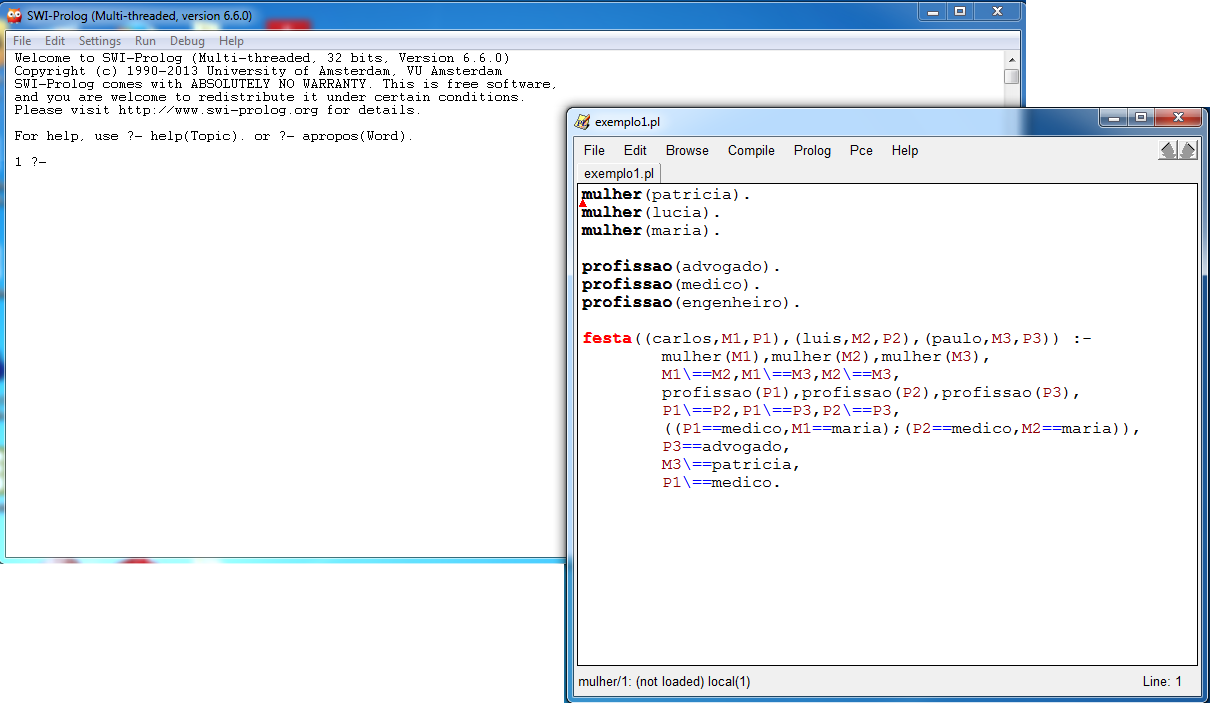
\includegraphics[width=9.5cm]{interface-swi-prolog}
	\end{center}
\end{frame}

\begin{frame}[fragile]{Exemplo de Programação Lógica (V)}
\begin{center}
{\bf exemplo1.pl}
\end{center}

\begin{scriptsize}
\begin{lstlisting}
profissao(medico).
profissao(engenheiro).
profissao(advogado).

mulher(maria).
mulher(lucia).
mulher(patricia).

festa((carlos, M1, P1), (luis, M2, P2), (paulo, M3, P3)) :-
     mulher(M1), mulher(M2), mulher(M3),
     M1\==M2,M1\==M3,M2\==M3,
     profissao(P1), profissao(P2), profissao(P3),
     P1\==P2,P1\==P3,P2\==P3,
     ((P1 == medico,M1 == maria);(P2 == medico, M2 == maria)),
     P3 == advogado,
     M3 \== patricia,
     P1 \== medico.	
\end{lstlisting}
\end{scriptsize}
\end{frame}

\begin{frame}[t]{Inferência PROLOG com Sentenças Abertas}
	\begin{itemize}
	\item O que nós acabamos de fazer foi uma inferência (em uma base de conhecimento) a partir de uma sentença aberta
	\item Ou seja, na prática o que o PROLOG foi construir uma enumeração de todas as possíveis combinações de particularização das variáveis envolvidas (produto cartesiano) e retornou aquela particularização que satisfez ao predicado inferido
	\item Notem que, dependendo do problema podem haver mais de uma particularização que satisfaz o problema. O Prolog irá apenas mostrar inicialmente a primeira destas. Caso se deseje ver outras possíveis respostas, use a tecla ``{\bf ;}'' (no tkEclipse há um botão na interface para isso)
	\item ``{\bf .}'' encerra o processo
	\end{itemize}
\end{frame}

\begin{frame}[t]{Inferência PROLOG com Sentenças Abertas}
	\begin{itemize}
	\item Mas como funciona o processo de determinação da particularização no Prolog ?
	\item Através de uma abordagem recursiva denominada {\bf backtracking} (retrocesso)
	\item Inicialmente, o sistema particulariza cada variável do predicado sendo inferido com a primeira opção disponível na base de conhecimento
	\item Em seguida, para a \underline{última} variável inferida, uma próxima particularização é determinada
	\item Quando não houverem mais particularizações possíveis para a última variável, então o processo é realizado para a penúltima variável de forma análoga (e assim por diante, para as demais variáveis)
	\end{itemize}
\end{frame}

\begin{frame}[fragile]{Inferência PROLOG com Sentenças Abertas}
\begin{center}
{\bf prodcartesiano.pl}
\end{center}

\begin{lstlisting}
a(1).
a(2).
a(3).
b(alfa).
b(beta).
b(gama).
produto(X,Y) :- a(X),b(Y).
\end{lstlisting}
\end{frame}


\begin{frame}[t]{Inferência PROLOG com Sentenças Abertas}
	\begin{itemize}
	\item Ao inferirmos a sentença ``{\bf produto(A,B).}'' obtemos como resultado todas as particularizações para as variáveis $A$ e $B$ que assumem os valores produzidos para as variáveis $X$ e $Y$ respectivamente: {\bf X/A Y/B}
	\item O resultado obtido é:
	\end{itemize}
	$$\begin{array}{l l}A = 1 & B = alfa \\ A = 1 & B = beta \\ A = 1 & B = gama\\ A = 2 & B = alfa \\ A = 2 & B = beta \\ A = 2 & B = gama\\ A = 3 & B = alfa \\ A = 3 & B = beta \\ A = 3 & B = gama \end{array}$$
\end{frame}


\begin{frame}[t]{Inferência PROLOG com Sentenças Abertas}
	\begin{itemize}
	\item Sempre que uma variável é particularizada por algum predicado, ela permanecerá particularizada pelo restante da interpretação ($\Phi$) daquele predicado (variáveis não mudam de valor durante uma interpretação)
	\item Neste caso, predicados que já tenham suas variáveis particularizadas se tornam `fatos' e são interpretadas pelo Prolog como proposições (V ou F)
	\end{itemize}
\end{frame}


\begin{frame}[fragile]{Inferência PROLOG com Sentenças Abertas}
\begin{center}
{\bf prodcartesiano2.pl}
\end{center}

\begin{lstlisting}
a(1).
a(2).
a(3).
b(1).
b(3).
b(5).
c(X,Y) :- a(Y), b(X).
produto(X,Y) :- a(X),b(Y),c(X,Y).
\end{lstlisting}

\begin{center}
Qual a sequência de particularizações para o predicado ``produto(A,B).'' ?
\end{center}
\end{frame}

\begin{frame}[t]{Prolog - Exercício (I)}
	\begin{enumerate}
	\item Traduzir o exercício dos caminhos e estradas visto em aula, para Prolog
	\item Repetir a inferência ``{\bf caminho(joinville, florianopolis).}'' para confirmar se a programação está correta
	\item Inferir outros caminhos (válidos e inválidos)
	\item Acrescentar novas cidades e estradas ao mapa original
	\end{enumerate}
\end{frame}

\begin{frame}[t]{Prolog - Exercício (II)}
	\begin{enumerate}
	\item Traduzir o exercício do soberano visto em aula, para Prolog
	\item Repetir a inferência ``{\bf odeia(marcos, cesar).}'' para confirmar se a programação está correta
	\end{enumerate}
\end{frame}

\begin{frame}[t]{Prolog - Exercício (III)}
	\begin{enumerate}
	\item Construir um programa em PL para descrever relações familiares em uma árvore genealógica
	\item Considere como fatos: homem, mulher, pai, casal
	\item \underline{Sugestão:} use sua própria família como exemplo
	\item Construa regras para descrever os seguintes predicados: irmão, irmã, avô, avó, tio, tia, primo, prima
	\end{enumerate}

	\vskip 0.3cm

	\begin{center}
	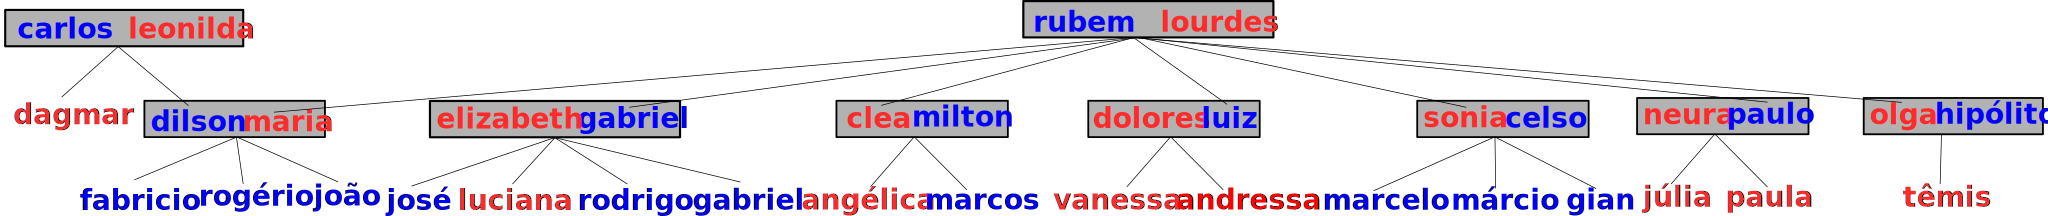
\includegraphics[width=\textwidth]{familia}
	\end{center}
\end{frame}

\begin{frame}[fragile]{Prolog - Exercício (III)}
\begin{center}
{\bf familia-pessoas.pl}
\end{center}

\begin{minipage}{0.4\textwidth}
\begin{tiny}
\begin{lstlisting}
homem(carlos).
homem(rubem).
homem(dilson).
homem(fabricio).
homem(rogerio).
homem(joao).
homem(gabriel).
homem(jose).
homem(rodrigo).
homem(gabrielzinho).
homem(milton).
homem(marcos).
homem(luiz).
homem(celso).
homem(marcelo).
homem(marcio).
homem(gian).
homem(paulo).
homem(hipolito).
\end{lstlisting}
\end{tiny}
\end{minipage}
\begin{minipage}{0.4\textwidth}
\begin{tiny}
\begin{lstlisting}
mulher(leonilda).
mulher(lourdes).
mulher(maria).
mulher(dagmar).
mulher(elizabeth).
mulher(luciana).
mulher(clea).
mulher(angelica).
mulher(dolores).
mulher(vanessa).
mulher(andressa).
mulher(sonia).
mulher(neura).
mulher(julia).
mulher(paula).
mulher(olga).
mulher(temis).
\end{lstlisting}
\end{tiny}
\end{minipage}
\end{frame}

\begin{frame}[fragile]{Prolog - Exercício (III)}
	\begin{center}
	{\bf familia-pais.pl}
	\end{center}

\begin{minipage}{0.4\textwidth}
\begin{tiny}
\begin{lstlisting}
pai(carlos, dilson).
pai(carlos, dagmar).
pai(dilson, fabricio).
pai(dilson, rogerio).
pai(dilson, joao).
pai(rubem, maria).
pai(rubem, gabriel).
pai(rubem, clea).
pai(rubem, luiz).
pai(rubem, sonia).
pai(rubem, paulo).
pai(rubem, olga).
pai(gabriel, jose).
pai(gabriel, luciana).
pai(gabriel, rodrigo).
pai(gabriel, gabrielzinho).
pai(milton, angelica).
pai(milton, marcos).
pai(luiz, vanessa).
pai(luiz, andressa).
pai(celso, marcelo).
pai(celso, marcio).
pai(celso, gian).
pai(paulo, julia).
pai(paulo, paula).
pai(hipolito, temis).
\end{lstlisting}
\end{tiny}
\end{minipage}
\begin{minipage}{0.4\textwidth}
\begin{tiny}
\begin{lstlisting}
casal(carlos, leonilda).
casal(dilson, maria).
casal(rubem, lourdes).
casal(gabriel, elizabeth).
casal(milton, clea).
casal(luiz, dolores).
casal(celso, sonia).
casal(paulo, neura).
casal(hipolito, olga).
\end{lstlisting}
\end{tiny}
\end{minipage}
\end{frame}

\begin{frame}[fragile]{Prolog - Exercício (III)}
	\begin{center}
	{\bf familia-relacoes.pl}
	\end{center}

\begin{minipage}{0.4\textwidth}
\begin{tiny}
\begin{lstlisting}
mae(X,Y) :- mulher(X), pai(W,Y), casal(W,X).
avo(X,Y) :- homem(X), pai(W,Y), pai(X,W).
avo(X,Y) :- homem(X), mae(W,Y), pai(X,W).
avoh(X,Y) :- mulher(X), pai(W,Y), mae(X,W).
avoh(X,Y) :- mulher(X), mae(W,Y), mae(X,W).
irmao(X,Y) :- homem(X), pai(W,X), pai(W,Y), X\==Y.
irma(X,Y) :- mulher(X), pai(W,X), pai(W,Y), X\==Y.
irmaos(X,Y) :- irmao(X,Y) ; irma(X,Y).
tio(X,Y) :- homem(X), pai(W,Y), irmao(X,W) .
tio(X,Y) :- homem(X), mae(W,Y), irmao(X,W).
tio(X,Y) :- homem(X), pai(W,Y), irma(Z,W), casal(X,Z).
tio(X,Y) :- homem(X), mae(W,Y), irma(Z,W), casal(X,Z).
tia(X,Y) :- mulher(X), pai(W,Y), irma(X,W) .
tia(X,Y) :- mulher(X), mae(W,Y), irma(X,W).
tia(X,Y) :- mulher(X), pai(W,Y), irmao(Z,W), casal(Z,X).
tia(X,Y) :- mulher(X), mae(W,Y), irmao(Z,W), casal(Z,X).
primo(X,Y) :- homem(X), pai(W,X), pai(T,Y), irmao(W,T).
primo(X,Y) :- homem(X), pai(W,X), mae(T,Y), irmao(W,T).
primo(X,Y) :- homem(X), mae(W,X), pai(T,Y), irma(W,T).
primo(X,Y) :- homem(X), mae(W,X), mae(T,Y), irma(W,T).
prima(X,Y) :- mulher(X), pai(W,X), pai(T,Y), irmao(W,T).
prima(X,Y) :- mulher(X), pai(W,X), mae(T,Y), irmao(W,T).
prima(X,Y) :- mulher(X), mae(W,X), pai(T,Y), irma(W,T).
prima(X,Y) :- mulher(X), mae(W,X), mae(T,Y), irma(W,T).
\end{lstlisting}
\end{tiny}
\end{minipage}
\end{frame}
